\documentclass[DaoFP]{subfiles}
\begin{document}
    \setcounter{chapter}{9}

    \chapter{Adjunctions(伴随)}

    一位雕塑家通过去除不相关的石头直到雕塑显现出来。一位数学家通过抽象掉不相关的细节直到模式显现出来。

    我们能够使用映射入(mapping-in)和映射出(mapping-out)属性来定义许多构造。这些属性可以紧凑地表示为同态集(hom-sets)之间的同构关系。这种自然同构的模式被称为伴随(adjunction),一旦被识别出来,它几乎无处不在。

    \section{The Currying Adjunction(柯里化伴随)}

    指数对象(exponential)的定义是一个经典的伴随的例子,它关联了映射出和映射入的关系。每一个从积(product)出的映射对应于一个唯一的映射入指数对象:
    \[  \mathcal{C}(e \times a, b ) \cong  \mathcal{C} (e, b^a)  \]
    在左侧,$b$对象充当了焦点;在右侧,$e$对象成为了观察者。

    我们可以发现有两个函子(functors)在起作用。它们都以$a$为参数。在左侧,我们有积函子$(- \times a)$应用于$e$。在右侧,我们有指数函子$(-)^a$应用于$b$。

    如果我们将这些函子写作:
    \[ L_a e = e \times a \]
    \[ R_a b = b^a \]
    那么同态集之间的自然同构
    \[ \mathcal{C}(L_a e, b) \cong \mathcal{C}(e, R_a b) \]
    就被称为它们之间的伴随。

    在具体操作中,这个同构告诉我们,给定一个映射$\phi \in \mathcal{C}(L_a e, b)$,就有一个唯一的映射$\phi^T \in \mathcal{C}(e, R_a b)$,反之亦然。这些映射有时被称为彼此的\emph{转置}(transpose)——这个术语借用了矩阵代数的名称。

    伴随的简写为$L \dashv R$。将积函子代入$L$,将指数函子代入$R$,我们可以简洁地将柯里化伴随写为:

    \[ (- \times a) \dashv (-)^a \]

    指数对象$b^a$有时被称为\index{internal hom}\emph{内部同态},记作$[a, b]$。这与\emph{外部同态}相对,外部同态是集合$\cat C (a, b)$。外部同态\emph{不是} $\cat C$中的对象(除非$\cat C$本身是$\Set$)。使用这个记号,柯里化伴随可以写为:
    \[  \mathcal{C}(e \times a, b) \cong  \mathcal{C} (e, [a, b])  \]
    在这个伴随成立的范畴被称为笛卡尔封闭范畴(cartesian closed category)。

    由于函数在每种编程语言中都起着核心作用,因此笛卡尔封闭范畴构成了所有编程模型的基础。我们将指数$b^a$解释为函数类型$a \to b$。

    这里,$e$起着外部环境的作用——在λ演算中对应$\Gamma$。$\cat C(\Gamma \times a, b)$中的态射被解释为在环境$\Gamma$中扩展了一个类型为$a$的变量的表达式。函数类型$a \to b$因此表示一个闭包(closure),它可能从其环境中捕获一个类型为$e$的值。

    顺便说一句,(小)范畴的范畴$\mathbf{Cat}$也是笛卡尔封闭的,这在乘积范畴和函子范畴之间的伴随中得到了反映,并使用了相同的内部同态记号:
    \[ \mathbf{Cat} (\cat A \times \cat B, \cat C) \cong \mathbf{Cat} (\cat A, [\cat B, \cat C]) \]
    这里,两个同态集都是自然变换的集合。

    \section{The Sum and the Product Adjunctions(和与积的伴随)}

    柯里化伴随关联了两个自函子(endofunctors),但伴随可以很容易地推广到在不同范畴之间的函子。我们先来看看一些例子。

    \subsection{The Diagonal Functor(对角函子)}

    和(sum)与积(product)类型是使用双射(bijections)定义的,其中一侧是一个单一的箭头,另一侧是一对箭头。一对箭头可以看作是积范畴(product category)中的单一箭头。

    为了探索这一思想,我们需要定义对角函子(diagonal functor)$\Delta$,这是一个从$\mathcal{C}$到$\mathcal{C} \times \mathcal{C}$的特殊映射。它将一个对象$x$复制成一对对象$\langle x, x \rangle$。它也将一个箭头$f$复制为$\langle f, f \rangle$。

    有趣的是,对角函子与我们之前看到的常函子(constant functor)有关。常函子可以被视为一个有两个变量的函子——它只是忽略了第二个变量。我们在Haskell定义中见过:
    \begin{haskell}
        data Const c a = Const c
    \end{haskell}

    为了看到两者之间的联系,让我们将积范畴$\mathcal{C} \times \mathcal{C}$视为函子范畴$[\mathbf{2}, \mathcal{C}]$,换句话说,是$\mathbf{Cat}$中的指数对象$\mathcal{C}^{\mathbf{2}}$。实际上,从$\mathbf{2}$(带有两个对象的简图范畴)的函子选取了一对对象——这等同于积范畴中的单一对象。

    一个从$\mathcal{C}$到$[\mathbf{2}, \mathcal{C}]$的函子可以被展开为$\mathcal{C} \times \mathbf{2} \to \mathcal{C}$。对角函子忽略了来自$\mathbf{2}$的第二个参数:无论第二个参数是$1$还是$2$,它做的事情是一样的。这正是常函子所做的。因此,我们为它们都使用了相同的符号$\Delta$。

    顺便提一下,这种论证可以轻松推广到任何索引范畴,而不仅仅是$\mathbf{2}$。

    \subsection{The Sum Adjunction(和伴随)}

    回想一下,和是通过其映射出属性定义的。$a + b$的所有箭头与分别从$a$和$b$出来的一对箭头一一对应。用同态集的术语,我们可以写成:
    \[  \mathcal{C} (a + b, x) \cong \mathcal{C}( a , x) \times \mathcal{C}( b , x)\]
    这里右边的乘积只是集合的笛卡尔乘积,即对的集合。此外,我们之前已经看到,这种双射在$x$上是自然的。

    我们知道一对箭头在积范畴中是一个单一箭头。因此,我们可以将右边的元素看作是在$\mathcal{C} \times \mathcal{C}$中的箭头,从对象$\langle a, b \rangle$到对象$\langle x, x \rangle$。后者可以通过对$x$作用的对角函子$\Delta$获得。我们有:

    \[  \mathcal{C} (a + b, x) \cong (\mathcal{C} \times \mathcal{C})( \langle a, b \rangle , \Delta x)\]
    这是两个不同范畴中同态集之间的双射。它满足自然性条件,因此它是一个自然同构。

    我们还可以在这里发现一对函子。在左边,我们有一个函子,它接受一对对象$\langle a, b \rangle$并生成它们的和$a + b$:
    \[ (+) \colon \mathcal{C} \times \mathcal{C} \to \mathcal{C}\]
    在右边,我们有对角函子$\Delta$,它朝相反的方向运行:
    \[ \Delta \colon \mathcal{C} \to  \mathcal{C} \times \mathcal{C} \]
    总之,我们有两个范畴之间的一对函子:
    \[
        \begin{tikzcd}
            \mathcal{C}
            \arrow[rr, bend right, "\Delta"']
            &&
            \mathcal{C} \times \mathcal{C}
            \arrow[ll, bend right, "(+)"']
        \end{tikzcd}
    \]
    以及同态集之间的同构:
    \[
        \begin{tikzcd}
            a + b
            \arrow[d, bend right, red, dashed]
            \arrow[d, dashed]
            \arrow[d, bend left, blue, dashed]
            &&
            \langle a , b \rangle
            \arrow[d, bend right, red, dashed]
            \arrow[d, dashed]
            \arrow[d, bend left, blue, dashed]
            \arrow[ll, bend right, "(+)"']
            \\
            x
            \arrow[rr, bend right, "\Delta"']
            &&
            \langle x, x \rangle
        \end{tikzcd}
    \]
    换句话说,我们有了伴随关系:
    \[ (+) \dashv \Delta \]

    \subsection{The Product Adjunction(积伴随)}

    我们可以将相同的推理应用于积的定义。这次我们有一个自然同构,关联的是一对箭头和一个映射入积。

    \[  \mathcal{C} (x, a) \times \mathcal{C}(x, b) \cong  \mathcal{C} (x, a \times b)  \]
    将一对箭头替换为积范畴中的箭头,我们得到:

    \[  (\mathcal{C} \times \mathcal{C})( \Delta x,  \langle a, b \rangle ) \cong  \mathcal{C} (x, a \times b)  \]
    这就是朝着相反方向运行的两个函子:
    \[
        \begin{tikzcd}
            \mathcal{C} \times \mathcal{C}
            \arrow[rr, bend right, "(\times)"']
            &&
            \mathcal{C}
            \arrow[ll, bend right, "\Delta"']
        \end{tikzcd}
    \]
    以及同态集之间的同构:

    \[
        \begin{tikzcd}
            \langle x, x \rangle
            \arrow[d, bend right, red, dashed]
            \arrow[d, dashed]
            \arrow[d, bend left, blue, dashed]
            &&
            x
            \arrow[d, bend right, red, dashed]
            \arrow[d, dashed]
            \arrow[d, bend left, blue, dashed]
            \arrow[ll, bend right, "\Delta"']
            \\
            \langle a , b \rangle
            \arrow[rr, bend right, "(\times)"']
            &&
            a \times b
        \end{tikzcd}
    \]
    换句话说,我们有了伴随关系:
    \[ \Delta \dashv (\times) \]

    \subsection{Distributivity(分配律)}

    在双笛卡尔封闭范畴(bicartesian closed category)中,积分配于和。我们已经使用通用构造看到了证明的一种方向。结合Yoneda引理,伴随关系给了我们更强大的工具来解决这个问题。

    我们希望证明以下自然同构:
    \[(b + c) \times a \cong b \times a + c \times a \]
    与其直接证明这个等式,我们将展示从两边映射出的所有映射到任意对象$x$是同构的:
    \[  \mathcal{C} ((b + c) \times a, x) \cong \mathcal{C}(b \times a + c \times a, x) \]
    左边是从积映射出,因此我们可以将柯里化伴随应用于它:
    \[  \mathcal{C} ((b + c) \times a, x) \cong \mathcal{C}(b + c, x^a) \]
    这给了我们一个从和映射出的映射,根据和伴随,它与两个映射的乘积同构:
    \[  \mathcal{C}(b + c, x^a) \cong \mathcal{C}(b, x^a) \times \mathcal{C}(c, x^a)\]
    现在我们可以对两个分量应用柯里化伴随的逆映射:
    \[  \mathcal{C}(b, x^a) \times \mathcal{C}(c, x^a) \cong \mathcal{C}(b \times a, x) \times \mathcal{C}(c \times a, x)\]
    使用和伴随的逆映射,我们得到最终结果:
    \[ \mathcal{C}(b \times a, x) \times \mathcal{C}(c \times a, x) \cong \mathcal{C}(b \times a + c \times a, x) \]

    这个证明中的每一步都是自然同构,因此它们的组合也是自然同构。通过Yoneda引理,分配律左侧和右侧形成的两个对象因此是同构的。

    这一陈述的一个更短的证明来自我们即将讨论的左伴随的性质。

    \section{Adjunction between Functors(函子之间的伴随)}

    通常,伴随关联了两个在两个范畴之间的相反方向的函子。左函子为
    \[ L \colon \mathcal{D} \to \mathcal{C}\]
    右函子为:
    \[ R \colon \mathcal{C} \to  \mathcal{D} \]
    伴随$L \dashv R$定义为两个同态集之间的自然同构。
    \[  \mathcal{C} (L x, y) \cong \mathcal{D}( x , R y)\]
    换句话说,我们有一组在$x$和$y$上自然的可逆函数集:
    \[ \phi_{x y} \colon  \mathcal{C} (L x, y) \to \mathcal{D}( x , R y) \]
    例如,$y$上的自然性意味着,对于任意$f \colon y \to y'$,下图是交换的:
    \[
        \begin{tikzcd}
            \mathcal{C}(L x, y)
            \arrow[d, leftrightarrow, "\phi_{x y}"]
            \arrow[r, "{\mathcal{C}(L x, f)}"]
            &
            \mathcal{C}(L x, y')
            \arrow[d, leftrightarrow, "\phi_{x y'}"]
            \\
            \mathcal{D}(x, R y)
            \arrow[r, "{\mathcal{D}(x, R f)}"]
            & \mathcal{D}(x, R y')
        \end{tikzcd}
    \]
    或者,考虑到同态函子的箭头提升与后合成(post-composition)相同:
    \[
        \begin{tikzcd}
            \mathcal{C}(L x, y)
            \arrow[d, leftrightarrow, "\phi_{x y}"]
            \arrow[r, "f \circ -"]
            &
            \mathcal{C}(L x, y')
            \arrow[d, leftrightarrow, "\phi_{x y'}"]
            \\
            \mathcal{D}(x, R y)
            \arrow[r, "R f \circ -"]
            & \mathcal{D}(x, R y')
        \end{tikzcd}
    \]
    双头箭头可以沿任意方向(使用$\phi^{-1}_{x y}$向上)遍历,因为它们是同构的组成部分。

    图示上,我们有两个函子:
    \[
        \begin{tikzcd}
            \mathcal{C}
            \arrow[rr, bend right, "R"']
            &&
            \mathcal{D}
            \arrow[ll, bend right, "L"']
        \end{tikzcd}
    \]
    并且,对于任意一对$x$和$y$,两个同构的同态集:
    \[
        \begin{tikzcd}
            L x
            \arrow[d, bend right, red, dashed]
            \arrow[d, dashed]
            \arrow[d, bend left, blue, dashed]
            &&
            x
            \arrow[d, bend right, red, dashed]
            \arrow[d, dashed]
            \arrow[d, bend left, blue, dashed]
            \arrow[ll, bend right, "L"']
            \\
            y
            \arrow[rr, bend right, "R"']
            &&
            R y
        \end{tikzcd}
    \]
    这些同态集来自两个不同的范畴,但集合就是集合。我们说$L$是$R$的左伴随,或者$R$是$L$的右伴随。

    在Haskell中,这可以简化为一个多参数类型类:
    \begin{haskell}
        class (Functor left, Functor right) => Adjunction left right where
        ltor :: (left x -> y) -> (x -> right y)
        rtol :: (x -> right y) -> (left x -> y)
    \end{haskell}
    在文件顶部需要以下指示:
    \begin{haskell}
    {-# language MultiParamTypeClasses #-}
    \end{haskell}

    因此,在双笛卡尔范畴中,和是对角函子的左伴随;积是其右伴随。我们可以非常简洁地写出这一关系(或者我们可以将其印在粘土中,作为楔形文字的现代版本):
    \[ (+) \dashv \Delta \dashv (\times) \]

    \begin{exercise}
        绘制见证伴随函数$\phi_{x y}$在$x$上自然性的交换图。
    \end{exercise}

    \begin{exercise}
        伴随公式左侧的同态集$\mathcal{C} (L x, y)$暗示$L x$可以被视为某个函子(共预层)的表示对象。这个函子是什么?提示:它将$y$映射到一个集合。这个集合是什么?
    \end{exercise}

    \begin{exercise}
        相应地,表示对象$a$对于预层$P$的定义是:
        \[P x \cong \mathcal{D}(x, a)\]
        在伴随公式中,$R y$是哪个预层的表示对象。
    \end{exercise}

    \section{Limits and Colimits as Adjunctions(极限与余极限作为伴随)}

    极限的定义也涉及同态集之间的自然同构:
    \[ [\cat J, \mathcal{C}](\Delta_x, D)  \cong \mathcal{C}(x, \text{Lim} D) \]
    左侧的同态集在函子范畴中。其元素是锥(cones),即常函子$\Delta_x$和图示函子$D$之间的自然变换。右侧的是$\mathcal{C}$中的同态集。

    在一个所有极限都存在的范畴中,我们有这两个函子之间的伴随:
    \[ \Delta_{(-)} \colon \mathcal{C} \to  [\cat J, \mathcal{C}] \]
    和:
    \[ \text{Lim}{(-)} \colon  [\cat J, \mathcal{C}] \to \mathcal{C} \]

    相应地,余极限由以下自然同构描述:
    \[ [\cat J, \mathcal{C}](D, \Delta_x)  \cong \mathcal{C}( \text{Colim} D, x) \]
    我们可以用一个简洁的公式表示这两个伴随:
    \[ \text{Colim} \dashv \Delta \dashv \text{Lim}\]

    特别地,由于积范畴$\cat C \times \cat C$等价于$\cat C^2$,或者函子范畴$[\mathbf{2}, \cat C]$,我们可以将积和余积重新表述为极限和余极限:
    \[ [\mathbf{2}, \cat C](\Delta_x, \langle a, b \rangle) \cong \cat C(x, a \times b) \]
    \[ \cat C( a + b, x) \cong [\mathbf{2}, \cat C]( \langle a, b \rangle, \Delta_x) \]
    这里$\langle a, b \rangle$表示一个图示,这是一个函子$D \colon \mathbf{2} \to \cat C$作用于$\mathbf{2}$的两个对象。

    \section{Unit and Counit of an Adjunction(伴随的单位元与伴随元)}

    我们通过比较箭头的相等性来比较它们,但我们更喜欢使用同构来比较对象。

    然而,当涉及到函子时,我们却遇到了问题。一方面,它们是函子范畴中的对象,因此同构是比较的方式;但另一方面,它们在$\mathbf{Cat}$中是箭头,所以可能直接比较它们的相等性也没什么问题?

    为了更清楚地理解这一困境,我们应该问自己\emph{为什么}我们要使用箭头的相等性。并不是因为我们喜欢相等性,而是因为在一个集合中,除了比较元素是否相等之外,我们无事可做。同态集中的两个元素要么相等要么不相等,仅此而已。

    但在$\mathbf{Cat}$中情况并非如此,正如我们所知,它是一个$2$-范畴。这里,同态集本身具有范畴的结构——即函子范畴。在$2$-范畴中,我们有箭头之间的箭头,因此特别地,我们可以定义箭头之间的同构。在$\mathbf{Cat}$中,这些同构就是函子之间的自然同构。

    然而,尽管我们有选择使用同构代替箭头相等性的选项,但$\mathbf{Cat}$中的范畴法则仍然表示为相等性。例如,函子$F$与恒等函子的复合是\emph{等于}$F$的,同样地,结合律也是如此。如果$2$-范畴中的法则严格满足,那么它被称为\emph{严格的}(strict),而$\mathbf{Cat}$就是一个严格$2$-范畴的例子。

    但就比较范畴而言,我们有更多的选择。范畴是$\mathbf{Cat}$中的对象,因此有可能将两个范畴的同构定义为一对函子$L$和$R$:
    \[
        \begin{tikzcd}
            \mathcal{C}
            \arrow[rr, bend right, "R"']
            \arrow[loop, "\text{Id}_{ \mathcal{C}} "']
            &&
            \mathcal{D}
            \arrow[ll, bend right, "L"']
            \arrow[loop, "\text{Id}_{ \mathcal{D}} "']
        \end{tikzcd}
    \]
    使得:
    \begin{align*}
        L \circ R = \text{Id}_{ \mathcal{C}} \\
        \text{Id}_{ \mathcal{D}} = R \circ L
    \end{align*}
    这个定义涉及函子的相等性。然而更糟糕的是,作用在对象上时,它涉及到对象的相等性:
    \begin{align*}
        L (R x) = x \\
        y = R (L y)
    \end{align*}
    这就是为什么更适合讨论一种更弱的范畴\emph{等价}(equivalence)的概念,其中相等性被替换为同构:
    \begin{align*}
        L \circ R \cong \text{Id}_{ \mathcal{C}} \\
        \text{Id}_{ \mathcal{D}} \cong R \circ L
    \end{align*}
    对于对象而言,范畴的等价意味着一个往返生成的对象与原始对象是同构的,而不是相等的。在大多数情况下,这正是我们所需要的。

    伴随也定义为一对相反方向的函子,因此有必要问一下往返的结果是什么。

    定义伴随的同构适用于任何一对对象$x$和$y$
    \[  \mathcal{C} (L x, y) \cong \mathcal{D}( x , R y)\]
    因此,特别地,如果我们将$y$替换为$L x$,那么我们得到:
    \[  \mathcal{C} (L x, L x) \cong \mathcal{D}( x , R (L x))\]
    我们现在可以使用Yoneda技巧,并在左侧选择恒等箭头$id_{L x}$。该同构将其映射到右侧的一个唯一箭头,我们将其称为$\eta_x$:
    \[ \eta_x \colon x \to R ( L x) \]
    不仅为每个$x$定义了这个映射,而且它在$x$上是自然的。自然变换$\eta$被称为伴随的\emph{单位元}(unit)。如果我们注意到左侧的$x$是恒等函子对$x$的作用,那么我们可以写成:
    \[ \eta \colon \text{Id}_{\mathcal{D}} \to R \circ L \]

    作为一个例子,我们来计算余积伴随的单位元:
    \[  \mathcal{C} (a + b, x) \cong (\mathcal{C} \times \mathcal{C})( \langle a, b \rangle , \Delta x)\]
    通过将$x$替换为$a + b$。我们得到:
    \[ \eta_{\langle a, b \rangle} \colon \langle a, b \rangle \to \Delta(a + b) \]
    这是一对箭头,它们正是两个注入$\langle \text{Left}, \text{Right} \rangle$。

    我们可以通过将$x$替换为$R y$来做一个类似的操作:
    \[  \mathcal{C} (L (R y), y) \cong \mathcal{D}( R y , R y)\]
    对应于右侧的恒等箭头,我们在左侧得到一个箭头:
    \[ \varepsilon_y \colon L (R y) \to y \]
    这些箭头形成了另一个自然变换,称为伴随的\emph{伴随元}(counit):
    \[ \varepsilon \colon L \circ R \to \text{Id}_{\mathcal{C}}  \]

    请注意,如果这两个自然变换是可逆的,它们将证明范畴的等价性。但即使它们不是,这种“半等价”在范畴论的上下文中仍然非常有趣。

    作为一个例子,我们来计算积伴随的伴随元:
    \[  (\mathcal{C} \times \mathcal{C})( \Delta x,  \langle a, b \rangle ) \cong  \mathcal{C} (x, a \times b)  \]
    通过将$x$替换为$a \times b$。我们得到:
    \[ \varepsilon_{\langle a, b \rangle} \colon \Delta (a \times b) \to \langle a, b \rangle \]
    这是一对箭头,它们正是两个投影$\langle \text{fst}, \text{snd} \rangle$。

    \begin{exercise}
        推导出余积伴随的伴随元和积伴随的单位元。
    \end{exercise}

    \subsection{Triangle Identities(三角恒等式)}

    我们可以使用单位元/伴随元对来形成伴随的一个等价定义。为此,我们首先从一对自然变换开始:
    \begin{align*}
        \eta \colon \text{Id}_{\mathcal{D}} \to R \circ L \\
        \varepsilon \colon L \circ R \to \text{Id}_{\mathcal{C}}
    \end{align*}
    并施加额外的\emph{三角恒等式}(triangle identities)。

    这些恒等式可以从伴随的标准定义推导出来,通过注意到$\eta$可以用来用复合$R \circ L$替换恒等函子,实际上让我们可以在任何适用恒等函子的地方插入$R \circ L$。

    类似地,$\varepsilon$可以用来消除复合$L \circ R$(即,将其替换为恒等)。

    因此,例如,从$L$开始:
    \[ L = L \circ \text{Id}_{\mathcal{D}} \xrightarrow{L \circ \eta} L \circ R \circ L \xrightarrow{\varepsilon \circ L} \text{Id}_{\mathcal{C}} \circ L = L \]
    在这里,我们使用了自然变换的水平组合,其中之一是恒等变换(也称为whiskering)。

    第一个三角恒等式是这种变换链结果为恒等自然变换的条件。图示上:

    \[
        \begin{tikzcd}
            L
            \arrow[r, "L \circ \eta"]
            \arrow[rd, "id_L"']
            & L \circ R \circ L
            \arrow[d, "\varepsilon \circ L"]
            \\
            & L
        \end{tikzcd}
    \]

    类似地,我们希望以下自然变换链也组合成恒等式:
    \[ R = \text{Id}_{\mathcal{D}} \circ R \xrightarrow{\eta \circ R} R \circ L \circ R \xrightarrow{R \circ \varepsilon} R \circ \text{Id}_{\mathcal{C}} = R \]
    或者,图示上:
    \[
        \begin{tikzcd}
            R
            \arrow[r, "\eta \circ R"]
            \arrow[rd, "id_R"']
            & R \circ L \circ R
            \arrow[d, "R \circ \varepsilon"]
            \\
            & R
        \end{tikzcd}
    \]

    事实证明,伴随还可以用满足三角恒等式的两个自然变换$\eta$和$\varepsilon$来定义:
    \begin{align*}
    (\varepsilon \circ L) \cdot (L \circ \eta) = id_L \\
    (R \circ \varepsilon) \cdot (\eta \circ R) = id_R
    \end{align*}

    通过这些, 可以很容易地恢复同态集的映射。例如,从箭头$f \colon x \to R y$开始,它是$\mathcal{D}( x , R y)$的一个元素。我们可以将其提升为
    \[L f \colon L x \to L (R y)\]
    然后我们可以使用$\eta$来将复合$L \circ R$压缩为恒等。结果是一个箭头$L x \to y$,它是$ \mathcal{C} (L x, y)$的一个元素。

    使用单位元和伴随元的伴随定义更加通用,因为它可以翻译到任意$2$-范畴设置。

    \begin{exercise}
        给定一个箭头$g \colon L x \to y$,使用$\varepsilon$和$R$是一个函子的事实来实现一个箭头$x \to R y$。提示:从对象$x$开始,看看你可以如何通过一个中途站到达$R y$。
    \end{exercise}

    \subsection{The Unit and Counit of the Currying Adjunction(柯里化伴随的单位元与伴随元)}

    让我们计算柯里化伴随的单位元和伴随元:
    \[  \mathcal{C}(e \times a, b ) \cong  \mathcal{C} (e, b^a)  \]
    如果我们将$b$替换为$e \times a$,我们得到
    \[  \mathcal{C}(e \times a, e \times a ) \cong  \mathcal{C} (e, (e \times a)^a)  \]
    对应于左侧的恒等箭头,我们在右侧得到了伴随的单位元:
    \[ \eta \colon e \to (e \times a)^a \]
    这是一个积构造器的柯里化版本。在Haskell中,我们将其写为:
    \begin{haskell}
        unit :: e -> (a -> (e, a))
        unit = curry id
    \end{haskell}

    伴随元更有趣。将$e$替换为$b^a$,我们得到:
    \[  \mathcal{C}(b^a \times a, b ) \cong  \mathcal{C} (b^a, b^a)  \]
    对应于右侧的恒等箭头,我们得到:
    \[ \varepsilon \colon b^a \times a \to b \]
    这就是函数应用箭头。

    在Haskell中:
    \begin{haskell}
        counit :: (a -> b, a) -> b
        counit = uncurry id
    \end{haskell}

    当伴随发生在两个自函子之间时,我们可以使用单位元和伴随元写一个替代的Haskell定义:
    \begin{haskell}
        class (Functor left, Functor right) =>
        Adjunction left right | left -> right, right -> left where
        unit   :: x -> right (left x)
        counit :: left (right x) -> x
    \end{haskell}
    另外的两个子句\hask{left -> right}和\hask{right -> left}告诉编译器,在使用伴随实例时,一个函子可以从另一个推导出来。这个定义需要以下编译扩展:
    \begin{haskell}
    {-# language MultiParamTypeClasses #-}
    {-# LANGUAGE FunctionalDependencies #-}
    \end{haskell}

    构成柯里化伴随的两个函子可以写成:
    \begin{haskell}
        data L r x = L (x, r)    deriving (Functor, Show)
        data R r x = R (r -> x)  deriving Functor
    \end{haskell}
    以及柯里化的\hask{Adjunction}实例:
    \begin{haskell}
        instance Adjunction (L r) (R r) where
        unit x = R (\r -> L (x, r))
        counit (L (R f, r)) = f r
    \end{haskell}
    第一个三角恒等式声明以下多态函数:
    \begin{haskell}
        triangle :: L r x -> L r x
        triangle = counit . fmap unit
    \end{haskell}
    是恒等的,第二个也是:
    \begin{haskell}
        triangle' :: R r x -> R r x
        triangle' = fmap counit . unit
    \end{haskell}
    注意,这两个函数需要使用功能依赖才能正确定义。三角恒等式无法在Haskell中表达,因此实现伴随的开发人员必须自己证明它们。
    \begin{exercise}
        测试柯里化伴随的第一个三角恒等式的一些例子。以下是一个例子:
        \begin{haskell}
            triangle (L (2, 'a'))
        \end{haskell}
    \end{exercise}

    \begin{exercise}
        你会如何测试柯里化伴随的第二个三角恒等式?提示:\hask{triangle'}的结果是一个函数,所以你无法直接显示它,但你可以调用它。
    \end{exercise}

    \section{Adjunctions Using Universal Arrows(使用泛箭的伴随)}

    我们已经看到了使用同态集的同构来定义伴随的方式,以及使用单位元/伴随元对来定义伴随的另一种方式。事实证明,只要满足某种普遍性条件,我们可以只使用该对中的一个元素来定义伴随。为了理解这一点,我们将构造一个新的范畴,其对象是箭头。

    我们之前见过一个这样的范畴的例子——切片范畴(slice category)$\cat C/ c$,它收集了所有汇聚于$c$的箭头。这样的范畴描述了从$\cat C$中每个可能的角度来看$c$对象的视图。

    \subsection{Comma Category(逗号范畴)}
    当处理一个伴随关系时:
    \[  \mathcal{C} (L d, c) \cong \mathcal{D}( d , R c)\]
    我们正在从由函子$L$定义的较窄视角观察对象$c$。可以将$L$视为定义了一个范畴$\cat D$在$\cat C$内部的模型。我们感兴趣的是从这个模型的角度来看$c$的视图。描述这个视图的箭头构成了逗号范畴$L/c$。

    \[
        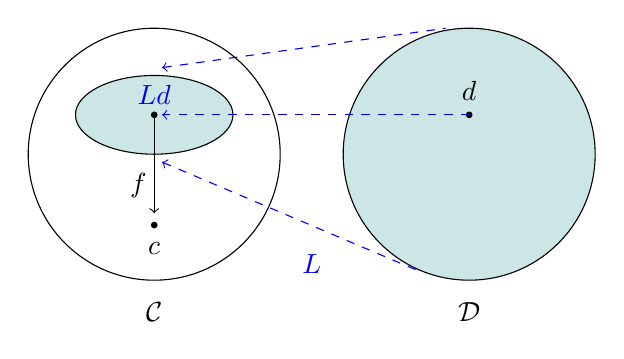
\begin{tikzpicture}
            \def\Xa{2.0};
            \def\Xb{-2.0};

            \def\Ytip{-0.9};
            \def\Yo{0.5}; % oval
            \def\Yb{-2.0}; % labels
            \draw (\Xa, 0)[fill=blue!50!green!20]  ellipse (1.6 and 1.6);
            \draw (\Xb , 0) ellipse (1.6 and 1.6);
            % oval
            \draw (\Xb , \Yo)[fill=blue!50!green!20] ellipse (1 and 0.5);

            % apex
            \filldraw (\Xb, \Ytip) circle (1pt);
            \node at ( \Xb, \Ytip - 0.3) { $c$ };

            % image
            \filldraw (\Xa, \Yo) circle (1pt);
            \node at ( \Xa, \Yo + 0.3) { $d$ };

            % middle of the cone
            \draw[->] (\Xb, \Yo) -- (\Xb, \Ytip + 0.15);
            \node at (\Xb - 0.2, \Ytip + 0.5) {$f$};
            % sides of the cone
            %\draw (\Xb, \Ytip) -- (\Xb + 0.95, \Yo - 0.15);
            %\draw (\Xb, \Ytip) -- (\Xb - 0.95, \Yo - 0.15);

            % categories
            \node at (\Xa, \Yb) { $\mathcal D$ };
            \node at (\Xb, \Yb) { $\mathcal C$ };
            \node[blue] at (0, \Yb + 0.6) { $L$ };

            % functor middle
            \filldraw (\Xb, \Yo) circle (1pt);
            \node[blue] at ( \Xb, \Yo + 0.25) { $L d$ };
            \draw[->, blue, dashed] (\Xa, \Yo) -- (\Xb + 0.1, \Yo);
            % functor
            \draw [<-, blue, dashed] (\Xb + 0.1, \Yo + 0.6)   --   (\Xa - 0.3, \Yo + 1.1);
            \draw [<-,blue, dashed] (\Xb + 0.1, \Yo - 0.6) -- (\Xa - 0.6, \Ytip - 0.6);
        \end{tikzpicture}
    \]

    逗号范畴$L/c$中的一个对象是一个对$\langle d, f \rangle$,其中$d$是$\cat D$的一个对象,$f \colon L d \to c$是$\cat C$中的一个箭头。

    从$\langle d, f \rangle$到$\langle d', f' \rangle$的态射是一个箭头$h \colon d \to d'$,它使得左边的图表交换:
    \[
        \begin{tikzcd}
            L d
            \arrow[rd, "f"']
            \arrow[rr, "L h"]
            && L d'
            \arrow[ld, "f'"]
            \\
            &c
        \end{tikzcd}
        \hspace{30pt}
        \begin{tikzcd}
            d
            \arrow[rr, "h"]
            && d'
        \end{tikzcd}
    \]

    \subsection{Universal Arrow(泛箭)}

    从$L$到$c$的泛箭被定义为逗号范畴$L/c$中的终对象。让我们展开这个定义。$L/c$中的终对象是一个对$\langle t, \tau \rangle$,它具有从任意对象$\langle d, f \rangle$的唯一态射。这样的态射是一个箭头$h \colon d \to t$,它满足交换条件:
    \[
        \begin{tikzcd}
            L d
            \arrow[rd, "f"']
            \arrow[rr, dashed, "L h"]
            && L t
            \arrow[ld, red, "\tau"]
            \\
            &c
        \end{tikzcd}
    \]
    换句话说,对于同态集$\cat C (L d, c)$中的任意$f$,在同态集$\cat D (d, t)$中有一个唯一的元素$h$,使得:
    \[ f = \tau \circ L h \]
    两个同态集之间的这种一对一映射暗示了潜在的伴随关系。

    \subsection{从伴随推导出的泛箭}

    让我们首先确认,当函子$L$有一个右伴随$R$时,对于每一个$c$,存在从$L$到$c$的一个泛箭。事实上,这个箭头由对$\langle R c, \varepsilon_c \rangle$给出,其中$\varepsilon$是伴随的伴随元。首先,伴随元的分量具有适用于逗号范畴$L/c$中对象的签名:
    \[ \varepsilon_c \colon L (R c) \to c \]

    我们想要证明$\langle R c, \varepsilon_c \rangle$是$L/c$中的终对象。也就是说,对于任意对象$\langle d, f \colon L d \to c \rangle$,存在一个唯一的$h \colon d \to R c$,使得$f = \varepsilon_c \circ L h$:
    \[
        \begin{tikzcd}
            L d
            \arrow[rd, "f"']
            \arrow[rr, dashed, "L h"]
            && L (R c)
            \arrow[ld, red, "\varepsilon_c"]
            \\
            &c
        \end{tikzcd}
    \]
    为了证明这一点,让我们写出$\phi_{d c}$作为$d$的函数的一个自然性条件:
    \[  \phi_{d c} \colon \mathcal{C} (L d, c) \to \mathcal{D}( d , R c)\]
    对于任意箭头$h \colon d \to d'$,下图必须交换:
    \[
        \begin{tikzcd}
            \mathcal{C}(L d', c)
            \arrow[d, leftrightarrow, "\phi_{d', c}"]
            \arrow[r, "- \circ L h"]
            &
            \mathcal{C}(L d, c)
            \arrow[d, leftrightarrow, "\phi_{d, c}"]
            \\
            \mathcal{D}(d', R c)
            \arrow[r, "- \circ h"]
            & \mathcal{D}(d, R c)
        \end{tikzcd}
    \]
    我们可以通过将$d'$设置为$R c$来使用Yoneda技巧。

    \[
        \begin{tikzcd}
            \mathcal{C}(L (R c), c)
            \arrow[d, leftrightarrow, "\phi_{R c, c}"]
            \arrow[r, "- \circ L h"]
            &
            \mathcal{C}(L d, c)
            \arrow[d, leftrightarrow, "\phi_{d, c}"]
            \\
            \mathcal{D}(R c, R c)
            \arrow[r, "- \circ h"]
            & \mathcal{D}(d, R c)
        \end{tikzcd}
    \]
    我们现在可以选择同态集$\cat D(R c, R c)$的特殊元素,即恒等箭头$id_{R c}$,并将其传播到其余的图表中。左上角变为$\varepsilon_c$,右下角变为$h$,右上角变为与$h$对应的箭头,我们称其为$f$:

    \[
        \begin{tikzcd}
            \varepsilon_c
            \arrow[d, leftrightarrow, "\phi_{R c, c}"]
            \arrow[r, maps to, "- \circ L h"]
            &
            f
            \arrow[d, leftrightarrow, "\phi_{d, c}"]
            \\
            id_{R c}
            \arrow[r, maps to, "- \circ h"]
            & h
        \end{tikzcd}
    \]
    然后,顶部的箭头给出了我们所寻找的等式$f = (- \circ L h) \varepsilon_c = \varepsilon_c \circ L h$。

    \subsection{从泛箭推导出的伴随}

    反过来说,结果更加有趣。如果对于每个$c$,我们都有从$L$到$c$的一个泛箭,即逗号范畴$L/c$中的终对象$\langle t_c, \varepsilon_c \rangle$,那么我们可以构造一个函子$R$,它是$L$的右伴随。该函子对对象的作用由$R c = t_c$给出,并且$\varepsilon_c$在$c$中自动是自然的,并且构成了伴随的伴随元。

    还有一个对偶的陈述:可以从泛箭$\eta_d$的族开始构造一个伴随,这些泛箭构成了逗号范畴$d/R$中的初始对象。

    这些结果将帮助我们证明Freyd的伴随函子定理。

    \section{伴随的性质}

    \subsection{左伴随保持余极限}

    我们将余极限定义为泛余锥。对于每个余锥——即从图式$D \colon \cat J \to \cat C$到常函子$\Delta_x$的自然变换——应该有一个从余极限$\text{Colim}\, D$到$x$的唯一分解态射。这个条件可以写为余锥集和特定同态集之间的一对一对应:
    \[ [\cat J, \mathcal{C}](D, \Delta_x)  \cong \mathcal{C}( \text{Colim} \, D, x) \]
    分解条件被编码在这个同构的自然性中。

    事实证明,余锥集是$\Set$中的一个对象,它本身是以下$\Set$值函子$F \colon \cat J \to \Set$的\emph{极限}:
    \[ F j = \cat C(D j, x) \]

    为了展示这一点,我们将从$F$的极限开始,并最终得到余锥集。您可能记得,一个$\Set$值函子的极限等于以单集$1$为顶点的锥的集合。在我们的例子中,每个这样的锥描述了从相应的同态集$\cat C(D j, x)$中选择态射:
    \[
        \begin{tikzcd}
            & 1
            \arrow[ddr, ""]
            \arrow[ddl, ""']
            \arrow[ddd, ""]
            \\
            \\
            \cat C( D j_1, x)
            \arrow[rr, red]
            \arrow[rd, red]
            && \cat C( D j_2, x)
            \arrow[dl, red]
            \\
            & \cat C( D j_3, x)
        \end{tikzcd}
    \]
    这些态射的目标都是相同的对象$x$,因此它们构成了以$x$为顶点的余锥的边。
    \[
        \begin{tikzcd}
            D j_1
            \arrow[rr, red]
            \arrow[dr, red]
            \arrow[dddr, ""']
            && D j_2
            \arrow[dl, red]
            \arrow[dddl, ""]
            \\
            & D j_3
            \arrow[dd, ""]
            \\
            \\
            & x
        \end{tikzcd}
    \]
    以$1$为顶点的锥的交换条件同时也是以$x$为顶点的这个余锥的交换条件。但这些正是集$[\cat J, \mathcal{C}](D, \Delta_x)$中的余锥。

    因此,我们可以用$\cat C(D-, x)$的极限替换原始的余锥集,以得到:
    \[ \text{Lim}\; \cat C (D-, x) \cong \cat C( \text{Colim}\,  D, x) \]
    同态函子的逆变同态函子有时记为:
    \[ h_x = \cat C(-, x) \]
    在这个记号中,我们可以写成:
    \[ Lim \, (h_x \circ D) \cong h_x (Colim \, D) \]
    作用于图式$D$的同态函子的极限同构于作用于该图式的余极限的同态函子。这通常被缩写为:同态函子保持余极限。(理解为逆变同态函子将余极限转化为极限。)

    保持余极限的函子称为\index{co-continuous functor}余连续函子。因此,逆变同态函子是余连续的。

    现在假设我们有伴随$L \dashv R$,其中$L \colon \cat C \to \cat D$,$R$反方向运行。我们想要证明左函子$L$保持余极限,即:
    \[ L (\text{Colim} \, D) \cong \text{Colim} (L \circ D) \]
    对于任何存在余极限的图式$D \colon \cat J \to \cat C$。

    我们将使用Yoneda引理来证明两边映射到任意$x$的映射是同构的:
    \[ \cat D( L (\text{Colim} \, D), x) \cong \cat D (\text{Colim} (L \circ D), x) \]
    我们将伴随应用于左边,以得到:
    \[ \cat D( L (\text{Colim} \, D), x) \cong \cat C (\text{Colim}\, D, R x) \]
    同态函子保持余极限给我们:
    \[ \cong \text{Lim}\; \cat C(D -, R x) \]
    再次使用伴随,我们得到:
    \[ \cong \text{Lim}\; \cat D((L \circ D) -, x) \]
    同态函子的第二次应用保持余极限给出了我们想要的结果:
    \[ \cong  \cat D((\text{Colim}\;(L \circ D), x) \]
    因为这对任何$x$都是成立的,所以我们得到了我们的结果。

    我们可以使用这个结果来重新表述我们在笛卡尔封闭范畴中的分配律的早期证明。我们使用了积是指数的左伴随的事实。左伴随保持余极限。余积是一个余极限,因此:
    \[(b + c) \times a \cong b \times a + c \times a \]
    这里,左函子是$L x = x \times a$,图式$D$选择一对对象$b$和$c$。

    \subsection{右伴随保持极限}

    使用对偶论证,我们可以证明右伴随保持极限,即:
    \[ R (\text{Lim}\, D) \cong \text{Lim}\, (R \circ D) \]

    我们首先证明同态函子保持极限。
    \[ \text{Lim}\; \cat C( x, D-) \cong \mathcal{C}(x, \text{Lim}\,D) \]
    这可以从一个论证得出,即定义极限的锥集同构于$\Set$值函子的极限:
    \[ F j = \cat C(x, D j) \]
    保持极限的函子称为\index{continuous functor}连续函子。

    为了证明给定的伴随$L \dashv R$,右函子$R \colon \cat D \to \cat C$保持极限,我们使用Yoneda论证:
    \[ \cat C(x, R (\text{Lim}\, D)) \cong \cat C (x, \text{Lim}\, (R \circ D)) \]
    实际上,我们有:
    \[ \cat C(x, R (\text{Lim}\, D)) \cong \cat D(L x, \text{Lim}\, D) \cong \text{Lim}\; \cat D(L x, D-) \cong \cat C(x, \text{Lim}\, (R \circ D))\]


    \section{Freyd的伴随函子定理}

    一般来说,函子是有损的——它们不可逆。在某些情况下,我们可以通过用“最佳猜测”替换丢失的信息来弥补这一点。如果我们以有组织的方式进行,我们最终会得到一个伴随。问题是:给定两个范畴之间的一个函子,在什么条件下我们可以构造出它的伴随?

    Freyd的伴随函子定理给出了这个问题的答案。起初,这似乎是一个涉及非常抽象构造的技术性定理,称为解集条件。我们稍后会看到,这个条件直接转化为一种编程技术,称为去函数化。

    在接下来的内容中,我们将重点放在构造一个函子$L \colon \cat D \to \cat C$的右伴随上。可以使用对偶推理来解决寻找函子$R \colon \cat C \to \cat D$的左伴随的相反问题。

    第一个观察是,由于伴随中的左函子保持余极限,我们必须假定我们的函子$L$保持余极限。这给了我们一个提示,即右伴随的构造依赖于在$\cat D$中构造余极限的能力,并能够通过某种方式将它们带回$\cat C$,使用$L$。

    我们可以要求$\cat D$中的所有余极限,无论大小,都存在,但这个条件太强了。即使是一个拥有所有余极限的小范畴也会自动成为预序——也就是说,在任何两个对象之间都不能有多个态射。

    但是让我们暂时忽略大小问题,看看如何为一个保持余极限的函子$L$定义右伴随,其源范畴$\cat D$是小的并且具有所有余极限,无论大小(因此它是一个预序)。

    \subsection{Freyd定理在预序中的应用}

    定义$L$的右伴随的最简单方法是为每个对象$c$构造一个从$L$到$c$的泛箭。这样的箭头是逗号范畴$L/c$中的终对象——这个范畴中的箭头起源于$L$的像,并汇聚于对象$c$。

    \[
        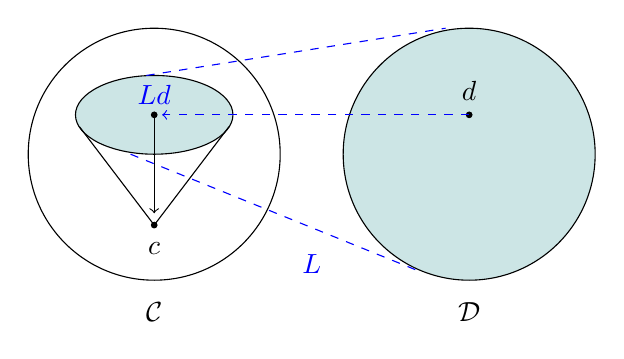
\begin{tikzpicture}
            \def\Xa{2.0};
            \def\Xb{-2.0};

            \def\Ytip{-0.9};
            \def\Yo{0.5}; % oval
            \def\Yb{-2.0}; % labels
            \draw (\Xa, 0)[fill=blue!50!green!20]  ellipse (1.6 and 1.6);
            \draw (\Xb , 0) ellipse (1.6 and 1.6);
            % oval
            \draw (\Xb , \Yo)[fill=blue!50!green!20] ellipse (1 and 0.5);

            % apex
            \filldraw (\Xb, \Ytip) circle (1pt);
            \node at ( \Xb, \Ytip - 0.3) { $c$ };

            % image
            \filldraw (\Xa, \Yo) circle (1pt);
            \node at ( \Xa, \Yo + 0.3) { $d$ };

            % middle of the cone
            \draw[->] (\Xb, \Yo) -- (\Xb, \Ytip + 0.15);
            % sides of the cone
            \draw (\Xb, \Ytip) -- (\Xb + 0.95, \Yo - 0.15);
            \draw (\Xb, \Ytip) -- (\Xb - 0.95, \Yo - 0.15);

            % categories
            \node at (\Xa, \Yb) { $\mathcal D$ };
            \node at (\Xb, \Yb) { $\mathcal C$ };
            \node[blue] at (0, \Yb + 0.6) { $L$ };

            % functor middle
            \filldraw (\Xb, \Yo) circle (1pt);
            \node[blue] at ( \Xb, \Yo + 0.25) { $L d$ };
            \draw[->, blue, dashed] (\Xa, \Yo) -- (\Xb + 0.1, \Yo);
            % functor
            \draw [blue, dashed] (\Xb - 0.1, \Yo + 0.5    )   --   (\Xa - 0.3, \Yo + 1.1);
            \draw [blue, dashed] (\Xb - 0.3, \Yo - 0.5) -- (\Xa - 0.6, \Ytip - 0.6);
        \end{tikzpicture}
    \]

    重要的观察是这个逗号范畴描述了$\cat C$中的一个余锥。这个余锥的基底由那些能够不受阻碍地看到$c$的对象构成。这些基底中的箭头是$L/c$中的态射。正是这些箭头构成了余锥的边。
    \[
        \begin{tikzcd}
            L d
            \arrow[rd, "f"']
            \arrow[rr, "L h"]
            && L d'
            \arrow[ld, "f'"]
            \\
            &c
        \end{tikzcd}
        \hspace{30pt}
        \begin{tikzcd}
            d
            \arrow[rr, "h"]
            && d'
        \end{tikzcd}
    \]

    然后可以将这个余锥的基底投影回$\cat D$。存在一个投影$\pi_c$,它将$L/c$中的每一对$(d, f)$映射回$d$,从而忽略了箭头$f$。它还将$L/c$中的每个态射映射到产生它的$\cat D$中的箭头。通过这种方式,$\pi_c$定义了一个在$\cat D$中的图式。这个图式的余极限存在,因为我们假设在$\cat D$中存在所有余极限。我们称这个余极限为$t_c$:
    \[ t_c = \text{colim}\; \pi_c \]

    \[
        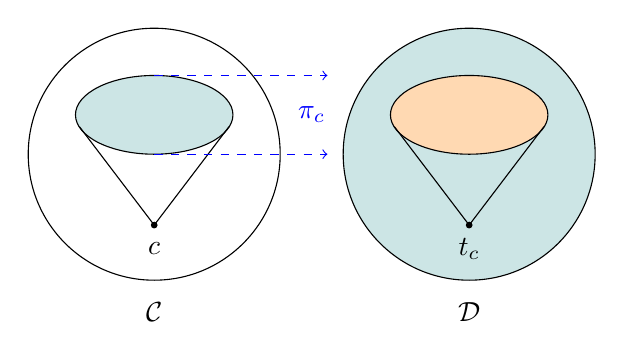
\begin{tikzpicture}
            \def\Xa{2.0};
            \def\Xb{-2.0};

            \def\Ytip{-0.9};
            \def\Yo{0.5}; % oval
            \def\Yb{-2.0}; % labels
            \draw (\Xa, 0)[fill=blue!50!green!20]   ellipse (1.6 and 1.6);
            \draw (\Xb , 0) ellipse (1.6 and 1.6);
            % oval
            \draw (\Xb , \Yo)[fill=blue!50!green!20]  ellipse (1 and 0.5);

            % apex
            \filldraw (\Xb, \Ytip) circle (1pt);
            \node at ( \Xb, \Ytip - 0.3) { $c$ };

            % sides of the cone
            \draw (\Xb, \Ytip) -- (\Xb + 0.95, \Yo - 0.15);
            \draw (\Xb, \Ytip) -- (\Xb - 0.95, \Yo - 0.15);

            % second oval
            \draw (\Xa , \Yo) [fill=orange!30]  ellipse (1 and 0.5);

            % apex
            \filldraw (\Xa, \Ytip) circle (1pt);
            \node at ( \Xa, \Ytip - 0.3) { $t_c$ };

            % sides of the cone
            \draw (\Xa, \Ytip) -- (\Xa + 0.95, \Yo - 0.15);
            \draw (\Xa, \Ytip) -- (\Xa - 0.95, \Yo - 0.15);

            % categories
            \node at (\Xa, \Yb) { $\mathcal D$ };
            \node at (\Xb, \Yb) { $\mathcal C$ };
            \node[blue] at (0, \Yo) { $\pi_c$ };

            % functor
            \draw [->, blue, dashed] (\Xb, \Yo + 0.5) --  (\Xb + 2.2, \Yo + 0.5);
            \draw [->, blue, dashed] (\Xb, \Yo - 0.5)  -- (\Xb + 2.2, \Yo - 0.5);
        \end{tikzpicture}
    \]

    让我们看看是否可以使用这个$t_c$来构造逗号范畴$L/c$中的终对象。我们必须找到一个箭头,我们称之为$\varepsilon_c \colon L t_c \to c$,使得对$\langle t_c, \varepsilon_c \rangle$在$L/c$中是终的。

    请注意,$L$将由$\pi_c$生成的图式映射回由$L/c$定义的余锥的基底。投影$\pi_c$只做了忽略这个余锥的边,而保留其基底。

    我们现在在$\cat C$中有两个余锥,它们具有相同的基底:一个顶点为$c$的原始余锥和一个通过对$\cat D$中的余锥应用$L$得到的新余锥。由于$L$保持余极限,新余锥的余极限是$L t_c$——即余极限$t_c$的像:

    \[ \text{colim} \; (L \circ \pi_c) = L ( \text{colim} \; \pi_c) = L t_c\]

    通过泛构造,我们推断出必须存在从余极限$L t_c$到$c$的唯一余锥态射。这个态射,我们称之为$\varepsilon_c$,使得所有相关的三角形交换。

    剩下要证明的是$\langle t_c, \varepsilon_c \rangle$是$L/c$中的终对象,也就是说,对于任意$\langle d, f \colon L d \to c \rangle$,存在一个唯一的逗号范畴态射$h \colon d \to t_c$,使得下图三角形交换:

    \[
        \begin{tikzcd}
            L d
            \arrow[rd, "f"']
            \arrow[rr, dashed, "L h"]
            && L t_c
            \arrow[ld, red, "\varepsilon_c"]
            \\
            &c
        \end{tikzcd}
    \]

    请注意,任何这样的$d$都自动成为由$\pi_c$生成的图式的一部分(它是$\pi_c$作用于$\langle d, f \rangle$的结果)。我们知道$t_c$是$\pi_c$图式的极限。因此,在极限余锥中,必定有一条从$d$到$t_c$的线。我们选择这条线作为我们的$h$。

    \[
        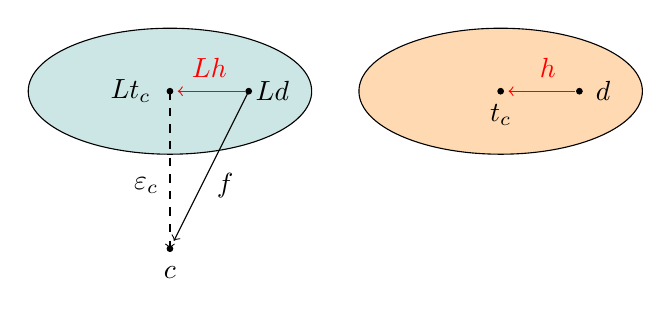
\begin{tikzpicture}
            \def\Xa{2.1};
            \def\Xb{-2.1};

            \def\Ytip{0};
            \def\Ybot{-2};
            \def\Yo{0}; % oval
            \def\Yf{-1.2}; % label
            % first oval
            \draw (\Xb , \Yo)[fill=blue!50!green!20]  ellipse (1.8 and 0.8);

            % second oval
            \draw (\Xa , \Yo) [fill=orange!30]  ellipse (1.8 and 0.8);

            % apex L tc
            \filldraw (\Xb, \Ytip) circle (1pt);
            \node at ( \Xb - 0.5, \Ytip) { $L t_c$ };

            % apex c
            \filldraw (\Xb, \Ybot) circle (1pt);
            \node at ( \Xb, \Ybot - 0.3) { $c$ };

            % sides of the cone L h
            \draw[red, ->]  (\Xb + 0.95, \Yo) -- (\Xb + 0.1, \Ytip);
            \node[red] at (\Xb + 0.5, \Ytip + 0.3) {$L h$};

            % apex tc
            \filldraw (\Xa, \Ytip) circle (1pt);
            \node at ( \Xa, \Ytip - 0.3) { $t_c$ };

            % sides of the cone h
            \draw [->, red] (\Xa + 0.95, \Yo) -- (\Xa + 0.1, \Ytip);
            \node[red] at ( \Xa + 0.6, \Ytip + 0.3) { $h$ };

            % d
            \filldraw (\Xa + 1, \Yo) circle (1pt);
            \node at ( \Xa + 1.3, \Yo) { $d$ };

            % L d
            \filldraw (\Xb + 1, \Yo) circle (1pt);
            \node at ( \Xb + 1.3, \Yo) { $L d$ };

            % f
            \draw[->] (\Xb + 1, \Yo) to (\Xb + 0.05, \Ybot + 0.1);
            \node at (\Xb + 0.7, \Yf) {$f$};

            % epsilon
            \draw[->, dashed] (\Xb, \Ytip) -- (\Xb, \Ybot);
            \node at (\Xb - 0.3, \Yf) {$\varepsilon_c$};

        \end{tikzpicture}
    \]
    然后,交换条件从$\varepsilon_c$作为两个余锥之间的态射得出。它是唯一的余锥态射,因为$\cat D$是一个预序。

    这证明了对于每一个$c$,都有一个从$L$到$c$的泛箭,因此我们有一个定义在对象上的函子$R c = t_c$,它是$L$的右伴随。

    \subsection{解集条件}

    前面证明的问题在于,大多数实际情况下的逗号范畴是大的:它们的对象并不构成一个集合。但也许我们可以通过选择较小但有代表性的对象和箭头集来近似逗号范畴?

    为了选择对象,我们可以使用从某个索引集$I$的映射。我们定义一组对象$d_i$,其中$i \in I$。由于我们试图近似逗号范畴$L/c$,我们选择带有箭头$f_i \colon L d_i \to c$的对象。

    逗号范畴的相关部分编码在满足交换条件的对象之间的态射中。我们可以尝试将此条件专门化为仅在我们的对象族内应用,但这还不够。我们必须找到一种方法来探测逗号范畴中的所有其他对象。

    为此,我们将交换条件重新解释为一个分解任意$f \colon L d \to c$通过某个对$\langle d_i, f_i \rangle$的配方:
    \[
        \begin{tikzcd}
            L d
            \arrow[rd, "f"']
            \arrow[rr, "L h"]
            && \textcolor{red}{L d_i}
            \arrow[ld, red, "f_i"]
            \\
            &c
        \end{tikzcd}
    \]

    一个\index{solution set}\emph{解集}是一个由索引集$I$索引的对$\langle d_i, f_i \colon L d_i \to c \rangle $的族,可以用来分解任意对$\langle d, f \colon L d \to c \rangle $。这意味着存在一个索引$i \in I$和一个箭头$h \colon d \to d_i$,它分解$f$:
    \[ f = f_i \circ L h \]

    表达这个属性的另一种方式是说在逗号范畴$L/c$中存在一个\index{weakly terminal set}\emph{弱终}的对象集。一个弱终集具有的属性是,对于范畴中的任何对象,都存在一个到该集中的至少一个对象的态射。

    我们之前已经看到,对于每个$c$,逗号范畴$L/c$中的终对象的存在足以定义伴随。事实证明,我们可以使用解集实现同样的目标。

    Freyd的伴随函子定理的假设规定我们有一个从一个小的完备范畴到另一个范畴的保持余极限的函子$L \colon \cat D \to \cat C$。这两个条件都与\emph{小}图式有关。如果我们可以为每个$c$选择一个解集$\langle d_i, f_i \colon L d_i \to c \rangle $,那么右伴随$R$存在。不同的$c$的解集可能不同。

    我们之前已经看到,在一个完备范畴中,弱终集的存在足以定义一个终对象。在我们的情况下,这意味着对于任何$c$,我们都可以构造从$L$到$c$的泛箭。而这足以定义整个伴随。

    伴随函子定理的对偶版本可用于构造左伴随。

    \subsection{去函数化}

    每种编程语言都允许我们定义函数,但并非所有语言都支持高阶函数(以函数为参数的函数,返回函数的函数,或由函数构造的数据类型)或匿名函数(又称lambda)。事实证明,即使在这种语言中,高阶函数也可以通过称为去函数化的过程来实现。这种技术基于伴随函子定理。此外,每当传递函数是不切实际的时候,例如在分布式系统中,都可以使用去函数化。

    去函数化背后的思想是函数类型被定义为积的右伴随。
    \[ \cat C(e \times a, b) \cong \cat C(e, b^a) \]
    伴随函子定理可以用来近似这个伴随。

    一般来说,任何有限的程序只能有有限数量的函数定义。这些函数(连同它们捕获的环境)形成了解集,我们可以用它来构造函数类型。在实践中,我们只为少数作为参数的函数或从其他函数返回的函数执行此操作。

    使用高阶函数的典型例子是继续传递风格。例如,下面是一个计算列表元素和的函数。但它不是返回和,而是使用结果调用一个继续\hask{k}:
    \begin{haskell}
        sumK :: [Int] -> (Int -> r) -> r
        sumK [] k = k 0
        sumK (i : is) k =
        sumK is (\s -> k (i + s))
    \end{haskell}
    如果列表为空,则该函数调用继续,和为零。否则,它以两个参数递归调用自己:列表\hask{is}的尾部和一个新的继续:
    \begin{haskell}
        \s -> k (i + s)
    \end{haskell}
    这个新的继续调用先前的继续\hask{k},并传递列表头的和及其参数\hask{s}(这是累积的和)。

    请注意,这个lambda是一个闭包:它是一个变量\hask{s}的函数,但它也可以访问来自其环境的\hask{k}和\hask{i}。

    要提取最终的和,我们用平凡的继续调用我们的递归函数,即恒等:
    \begin{haskell}
        sumList :: [Int] -> Int
        sumList as = sumK as (\i -> i)
    \end{haskell}

    匿名函数很方便,但没有什么能阻止我们使用命名函数。然而,如果我们想要将继续提取出来,我们必须明确传递环境。

    例如,我们可以替换我们的第一个lambda:
    \begin{haskell}
        \s -> k (i + s)
    \end{haskell}
    用函数\hask{more},但我们必须显式传递对\hask{(i, k)}作为类型\hask{(Int, Int -> r)}的环境:
    \begin{haskell}
        more :: (Int, Int -> r) -> Int -> r
        more (i, k) s = k (i + s)
    \end{haskell}
    另一个lambda,恒等,使用空环境,因此它变为:
    \begin{haskell}
        done :: Int -> Int
        done i = i
    \end{haskell}
    以下是使用这两个命名函数的算法实现:
    \begin{haskell}
        sumK' :: [Int] -> (Int -> r) -> r
        sumK' [] k = k 0
        sumK' (i : is) k =
        sumK' is (more (i, k))
    \end{haskell}

    \begin{haskell}
        sumList :: [Int] -> Int
        sumList is = sumK' is done
    \end{haskell}

    事实上,如果我们只对计算和感兴趣,我们可以将多态类型\hask{r}替换为\hask{Int},而不做其他更改。

    这个实现仍然使用高阶函数。为了消除它们,我们必须分析传递函数作为参数的含义。这样的函数只能以一种方式使用:可以将其应用于其参数。函数类型的这个属性表示为柯里化伴随的伴随元:
    \[ \varepsilon \colon b^a \times a \to b \]
    或者,在Haskell中,表示为一个高阶函数:
    \begin{haskell}
        apply :: (a -> b, a) -> b
    \end{haskell}
    这次我们有兴趣从第一个原理构造伴随元。我们已经看到,这可以通过逗号范畴实现。在我们的例子中,积函子$L_a = (-) \times a$的逗号范畴的一个对象是一个对
    \[(e, f \colon (e \times a) \to b) \]
    或者,在Haskell中:
    \begin{haskell}
        data Comma a b e = Comma e ((e, a) -> b)
    \end{haskell}
    这个范畴中$(e, f)$和$(e', f')$之间的态射是一个箭头$h \colon e \to e'$,它满足交换条件:
    \[ f' \circ h = f \]
    我们将这个态射解释为“缩减”环境$e$到$e'$。箭头$f'$能够使用由$h (e)$给出的可能较小的环境产生相同类型为$b$的输出。例如,$e$可能包含与从$a$计算$b$无关的变量,而$h$将它们投影出去。

    \[
        \begin{tikzcd}
            e \times a
            \arrow[rd, "f"']
            \arrow[rr, "h \times a"]
            && e' \times a
            \arrow[ld, "f'"]
            \\
            &b
        \end{tikzcd}
        \hspace{30pt}
        \begin{tikzcd}
            e
            \arrow[rr, "h"]
            && e'
        \end{tikzcd}
    \]


    事实上,我们在定义\hask{more}和\hask{done}时执行了这种类型的缩减。原则上,我们可以将尾部\hask{is}传递给这两个函数,因为它在调用点是可访问的。但我们知道它们不需要它。

    使用Freyd的定理,我们可以将函数对象$a \to b$定义为由逗号范畴定义的图式的余极限。这样的余极限本质上是所有环境的巨大余积,模态射的识别。这种识别将$a \to b$所需的环境减少到最低限度。

    在我们的例子中,我们感兴趣的继续是函数\hask{Int -> Int}。事实上,我们并不想生成通用的函数类型\hask{Int -> Int};只是要容纳我们的两个函数\hask{more}和\hask{done}的最小函数。我们可以通过创建一个非常小的解集来实现它。

    在我们的例子中,解集由对$(e_i, f_i \colon e_i \times a \to b)$组成,使得任何对$(e, f \colon e \times a \to b)$都可以通过其中一个$f_i$的分解。更确切地说,我们感兴趣的唯一两个环境是\hask{(Int, Int ->Int)}用于\hask{more},以及空环境\hask{()}用于\hask{done}。

    原则上,我们的解集应该允许分解逗号范畴的每个对象,即类型为:
    \begin{haskell}
        (e, (e, Int) -> Int)
    \end{haskell}
    但这里我们只对两个特定函数感兴趣。同样,我们并不关心表示的唯一性,因此,我们将使用所有感兴趣环境的余积(如我们在伴随函子定理中所做的),而不是使用余极限。我们最终得到了以下数据类型,它是我们感兴趣的两个环境\hask{()}和\hask{(Int, Int -> Int)}的和。我们最终得到了以下类型:
    \begin{haskell}
        data Kont = Done | More Int Kont
    \end{haskell}
    请注意,我们递归地将环境的\hask{Int->Int}部分编码为\hask{Kont}。因此,我们还消除了使用函数作为数据构造函数参数的需要。

    如果仔细观察这个定义,你会发现它是一个\hask{Int}列表的定义,模一些重命名。每次调用\hask{More}都会在\hask{Kont}堆栈上推送另一个整数。这个解释与我们的直觉一致,即递归算法需要某种运行时堆栈。

    我们现在准备实现我们的伴随元的近似。它由两个函数的主体组成,理解是递归调用也通过\hask{apply}:
    \begin{haskell}
        apply :: (Kont, Int) -> Int
        apply (Done, i) = i
        apply (More i k, s) = apply (k, i + s)
    \end{haskell}
    将此与我们之前的比较:
    \begin{haskell}
        done i = i
        more (i, k) s = k (i + s)
    \end{haskell}


    现在可以重写我们的主要算法,而不使用任何高阶函数或lambdas:
    \begin{haskell}
        sumK'' :: [Int] -> Kont -> Int
        sumK'' [] k = apply (k, 0)
        sumK'' (i : is) k = sumK'' is (More i k)
    \end{haskell}

    \begin{haskell}
        sumList'' is = sumK'' is Done
    \end{haskell}

    去函数化的主要优势在于它可以在分布式环境中使用。远程函数的参数,只要它们是数据结构而不是函数,就可以序列化并通过网络传递。所需的只是接收者可以访问\hask{apply}。

    \section{自由/遗忘伴随(Free/Forgetful Adjunctions)}
    在伴随关系中,两种函子扮演着不同的角色:伴随关系的图示并不是对称的。没有什么比自由/遗忘伴随关系更能说明这一点了。

    遗忘函子(forgetful functor)是指“遗忘”了其源范畴某些结构的函子。这并不是一个严格的定义,但在大多数情况下,遗忘了哪些结构是显而易见的。通常,目标范畴只是集合范畴($\mathbf{Set}$),这被认为是没有结构的典范。在这种情况下,遗忘函子的结果被称为“底层集合”(underlying set),而该函子本身通常称为$U$。

    更确切地说,我们说一个函子遗忘了\emph{结构},如果它的同态集的映射不是满射的,即在目标同态集中有些箭头在源同态集中没有对应的箭头。直观上,这意味着源范畴中的箭头具有某些要保留的结构,所以它们的数量较少;而在目标范畴中这种结构是不存在的。

    遗忘函子的左伴随函子被称为\emph{自由函子}(free functor)。

    \[
        \begin{tikzcd}
            F x
            \arrow[d, bend right, red, dashed]
            \arrow[d, dashed]
            \arrow[d, bend left, blue, dashed]
            &&
            x
            \arrow[d, bend right, red, dashed]
            \arrow[d, dashed]
            \arrow[d, bend left, blue, dashed]
            \arrow[ll, bend right, "F"']
            \\
            y
            \arrow[rr, bend right, "U"']
            &&
            U y
        \end{tikzcd}
    \]

    自由/遗忘伴随的一个经典例子是自由幺半群(free monoid)的构造。

    \subsection{幺半群范畴(The Category of Monoids)}
    在一个幺半范畴$\mathcal{C}$中,幺半群构成自己的范畴$\mathbf{Mon}(\mathcal{C})$。它的对象是幺半群,而它的箭头是保留幺半结构的$\mathcal{C}$中的箭头。

    下图解释了从一个幺半群$(M_1, \eta_1, \mu_1)$到另一个幺半群$(M_2, \eta_2, \mu_2)$的幺半群态射$f$的含义:

    \[
        \begin{tikzcd}
            & M_1
            \arrow[dd, "f"]
            & M_1 \otimes M_1
            \arrow[l, "\mu_1"]
            \arrow[dd, "f \otimes f"]
            \\
            I
            \arrow[ru, "\eta_1"]
            \arrow[rd, "\eta_2"']
            \\
            & M_2
            & M_2 \otimes M_2
            \arrow[l, "\mu_2"]
        \end{tikzcd}
    \]

    幺半群态射$f$必须将单位映射为单位,即:
    \[ f \circ \eta_1 = \eta_2 \]
    并且它必须将乘法映射为乘法:
    \[ f \circ \mu_1 = \mu_2 \circ (f \otimes f)\]

    请记住,张量积$\otimes$是函子性的,因此它可以提升箭头对,如$f \otimes f$。

    特别地,范畴$\mathbf{Set}$是单积范畴,具有笛卡尔积和提供单积结构的终对象。

    具体来说,$\mathbf{Set}$中的幺半群是带有附加结构的集合。它们构成自己的范畴$\mathbf{Mon}(\mathbf{Set})$,并且有一个遗忘函子$U$,它简单地将幺半群映射为其元素的集合。当我们说一个幺半群是一个集合时,我们指的是它的底层集合。

    \subsection{自由幺半群(Free Monoid)}

    我们要构造自由函子
    \[ F \colon \mathbf{Set} \to \mathbf{Mon}(\mathbf{Set})\]
    它是遗忘函子$U$的伴随函子。

    我们从一个任意集合$X$和一个任意幺半群$m$开始。在伴随关系的右侧,我们有从$X$到$U m$的函数集。在左侧,我们有一个从$F X$到$m$的高度受约束的保结构幺半群态射集。如何使这两个同态集同构呢?

    在$\mathbf{Mon}(\mathbf{Set})$中,幺半群是元素的集合,幺半群态射是这些集合之间的函数,满足附加约束:保留单位和乘法。

    另一方面,$\mathbf{Set}$中的箭头只是没有附加约束的函数。因此,一般来说,幺半群之间的箭头比它们底层集合之间的箭头要少。

    \[
        \begin{tikzcd}
            F X
            \arrow[d, bend right, red, dashed]
            \arrow[d, dashed]
            \arrow[d, bend left, blue, dashed]
            &&
            X
            \arrow[d, bend right, red, dashed]
            \arrow[d, dashed]
            \arrow[d, bend left, blue, dashed]
            \arrow[ll, bend right, "F"']
            \\
            m
            \arrow[rr, bend right, "U"']
            &&
            U m
        \end{tikzcd}
    \]

    这里的想法是:如果我们想要箭头之间有一一对应,我们希望$F X$比$X$大得多。这样一来,从$F X$到$m$的函数会多得多——即使在剔除那些不保留结构的函数后,我们仍然有足够多的函数可以匹配每一个$f \colon X \to U m$。

    我们将从集合$X$开始构造幺半群$F X$,并在此过程中添加越来越多的元素。我们将初始集合$X$称为$F X$的\index{generators of a monoid}\emph{生成元}。我们将从原始函数$f$开始,逐步扩展它,使其作用于越来越多的元素,从而构造幺半群态射$g \colon F X \to m$。

    在生成元$x \in X$上,$g$的作用与$f$相同:
    \[ g x = f x \]

    由于$F X$应该是一个幺半群,因此它必须有一个单位。我们不能选择一个生成元作为单位,因为这会对由$f$固定的$g$部分施加约束——它必须将该生成元映射为$m$的单位$e'$。所以我们只需向$F X$中添加一个额外的元素$e$,并称之为单位。我们通过将$g$映射到$m$的单位$e'$来定义$g$在它上的作用:
    \[ g e = e' \]

    我们还必须定义$F X$中的幺半乘法。让我们从两个生成元$a$和$b$的乘积开始。乘法的结果不能是另一个生成元,因为这同样会对$f$已经固定的$g$部分施加约束——乘积必须映射为乘积。因此,我们必须将生成元的所有乘积都作为$F X$中的新元素。同样,$g$在这些乘积上的作用是固定的:
    \[ g (a \cdot b)  = g a \cdot g b\]

    继续这种构造,任何新的乘法都会产生$F X$的一个新元素,除非它可以通过应用幺半群定律简化为一个已有的元素。例如,新单位$e$乘以生成元$a$必须等于$a$。但我们已经确保$e$映射为$m$的单位,因此乘积$g e \cdot g a$自动等于$g a$。

    另一种看待此构造的方法是将集合$X$视为字母表。然后,$F X$的元素是由此字母表中的字符组成的字符串。生成元是单字母字符串,如“$a$”、“$b$”等。单位是一个空字符串“”。乘法是字符串连接,所以“$a$”乘以“$b$”是一个新字符串“$ab$”。连接是自动的结合的和单位的,空字符串作为单位。

    自由函子背后的直觉是它们“自由地”生成结构,就像“没有额外约束”一样。它们还以懒惰的方式进行:它们记录操作,而不是执行操作。它们创建了特定领域的通用程序,可以由特定的解释器稍后执行。

    自由幺半群“记住了稍后进行乘法”。它将乘法的参数存储在字符串中,但不执行乘法。它只允许根据通用幺半群定律简化其记录。例如,它不必存储乘以单位的指令。它也可以“跳过括号”,因为它是结合的。

    \begin{exercise}
        自由幺半群伴随$F \dashv U$的单位元(unit)和伴随元(counit)是什么?
    \end{exercise}

    \subsection{编程中的自由幺半群(Free Monoid in Programming)}

    在Haskell中,幺半群通过以下类型类定义:
    \begin{haskell}
        class Monoid m where
        mappend :: m -> m -> m
        mempty  :: m
    \end{haskell}
    这里,\hask{mappend}是从积映射到映射的柯里化形式:\hask{(m, m) -> m}。元素\hask{mempty}对应于从终对象(单积范畴的单位元)的箭头,或简单地说,是\hask{m}的一个元素。

    由某种类型\hask{a}生成的自由幺半群,即作为生成元的集合,由列表类型\hask{[a]}表示。空列表作为单位;幺半群乘法实现为列表连接,传统上写成中缀形式:
    \begin{haskell}
    (++) :: [a] -> [a] -> [a]
    (++) []     ys = ys
    (++) (x:xs) ys = x : xs ++ ys
    \end{haskell}
    列表是\hask{Monoid}的一个实例:
    \begin{haskell}
        instance Monoid [a] where
        mempty = []
        mappend = (++)
    \end{haskell}

    要证明它是一个自由幺半群,我们必须能够从\hask{a}的列表构造一个到任意幺半群\hask{m}的幺半群态射,前提是我们有一个(不受约束的)从\hask{a}到(\hask{m}的底层集合)的映射。我们不能在Haskell中表达这一切,但我们可以定义如下函数:
    \begin{haskell}
        foldMap :: Monoid m => (a -> m) -> ([a] -> m)
        foldMap f = foldr mappend mempty . fmap f
    \end{haskell}
    此函数使用\hask{f}将列表元素转换为幺半群值,然后使用\hask{mappend}折叠它们,从单位\hask{mempty}开始。

    很容易看出,空列表映射为幺半群的单位。也不难看出,两个列表的连接映射为结果的幺半积。因此,确实,\hask{foldMap}是一个幺半群态射。

    根据自由幺半群作为领域特定乘法程序的直觉,\hask{foldMap}为该程序提供了一个\emph{解释器}。它执行所有已延迟的乘法操作。请注意,取决于具体幺半群和函数\hask{f}的选择,相同的程序可以用许多不同的方式进行解释。

    我们将在关于代数的章节中回到作为列表的自由幺半群。

    \begin{exercise}
        编写一个程序,接受一个整数列表,并以两种不同的方式对其进行解释:一次使用整数的加法幺半群,一次使用整数的乘法幺半群。
    \end{exercise}

    \section{伴随的范畴(The Category of Adjunctions)}
    我们可以通过利用定义它们的函子的组合来定义伴随的组合。如果两个伴随$L \dashv R$和$L' \dashv R'$,它们共享中间的范畴,则它们是可组合的:
    \[
        \begin{tikzcd}
            \mathcal{C}
            \arrow[rr, bend right, "R'"']
            &&
            \mathcal{D}
            \arrow[ll, bend right, "L'"']
            \arrow[rr, bend right, "R"']
            &&
            \mathcal{E}
            \arrow[ll, bend right, "L"']
        \end{tikzcd}
    \]
    通过组合函子,我们得到一个新的伴随$(L' \circ L) \dashv (R \circ R')$。

    实际上,让我们考虑同态集:
    \[ \mathcal{C}(L' (L e), c) \]
    使用$L' \dashv R'$伴随,我们可以将$L'$转移到右侧,使其成为$R'$:
    \[ \mathcal{D}(L e, R' c) \]
    并且使用$L \dashv R$我们可以类似地将$L$转移:
    \[ \mathcal{E}( e, R(R' c)) \]
    结合这两个同构,我们得到复合伴随:
    \[ \mathcal{C}((L' \circ L) e, c) \cong \mathcal{E}( e, (R \circ R') c)\]

    由于函子组合是结合的,伴随的组合也是结合的。很容易看出,一对恒等函子形成一个平凡的伴随,作为伴随组合的恒等。因此,我们可以定义一个范畴$\mathbf{Adj}(\mathbf{Cat})$,其中对象是范畴,箭头是伴随(按照惯例,指向左伴随的方向)。

    伴随可以纯粹用函子和自然变换定义,也就是2-范畴$\mathbf{Cat}$中的1-态射和2-态射。$\mathbf{Cat}$没有什么特别之处,实际上伴随可以在任何2-范畴中定义。此外,伴随的范畴本身就是一个2-范畴。

    \section{抽象的层次(Levels of Abstraction)}

    范畴论是关于组织我们的知识的。特别是,它可以应用于范畴论知识本身。因此,我们在范畴论中看到很多抽象层次的混合。在一个层次上看到的结构可以组合成更高层次的结构,这些结构展示了更高层次的结构,依此类推。

    在编程中,我们习惯于构建抽象层次。值被分组为类型,类型被分组为种类。操作值的函数与操作类型的函数被区别对待。我们通常使用不同的语法来分隔抽象层次。在范畴论中并非如此。

    从范畴论的角度来看,一个集合可以被描述为一个离散范畴。集合的元素是该范畴的对象,除了强制性的恒等态射外,它们之间没有箭头。

    然后,同一个集合可以在范畴$\mathbf{Set}$中被视为一个对象。该范畴中的箭头是集合之间的函数。

    范畴$\mathbf{Set}$,反过来,是范畴$\mathbf{Cat}$中的一个对象。$\mathbf{Cat}$中的箭头是函子。

    任意两个范畴$\mathcal{C}$和$\mathcal{D}$之间的函子是函子范畴$[\mathcal{C}, \mathcal{D}]$中的对象。该范畴中的箭头是自然变换。

    我们可以定义函子范畴之间的函子、积范畴、对偶范畴,依此类推,无限延伸。

    完成这一循环,每个范畴中的同态集都是集合。我们可以定义它们之间的映射和同构,跨越不同的范畴。由于我们可以比较不同范畴中的同态集,因此伴随关系是可能的。


\end{document}